%----------------------------------------------Modelo de Información de Estructura Educativa
\section{Modelo Estructural de Estructura Educativa}
En la figura \ref{fig:infoEstructuraEducativa} se puede observar un modelado de los datos que serán utilizados en el \refElem{Calmecac} para la creación de horarios(grupos, profesores y determinación de espacios para impartir una clase) así como para habilitar a los profesores la selección de unidades de aprendizaje que desea impartir si la \refElem{UnidadAcademica} utiliza esté formato.

\begin{figure}[hbtp!]
	\begin{center}
		\fbox{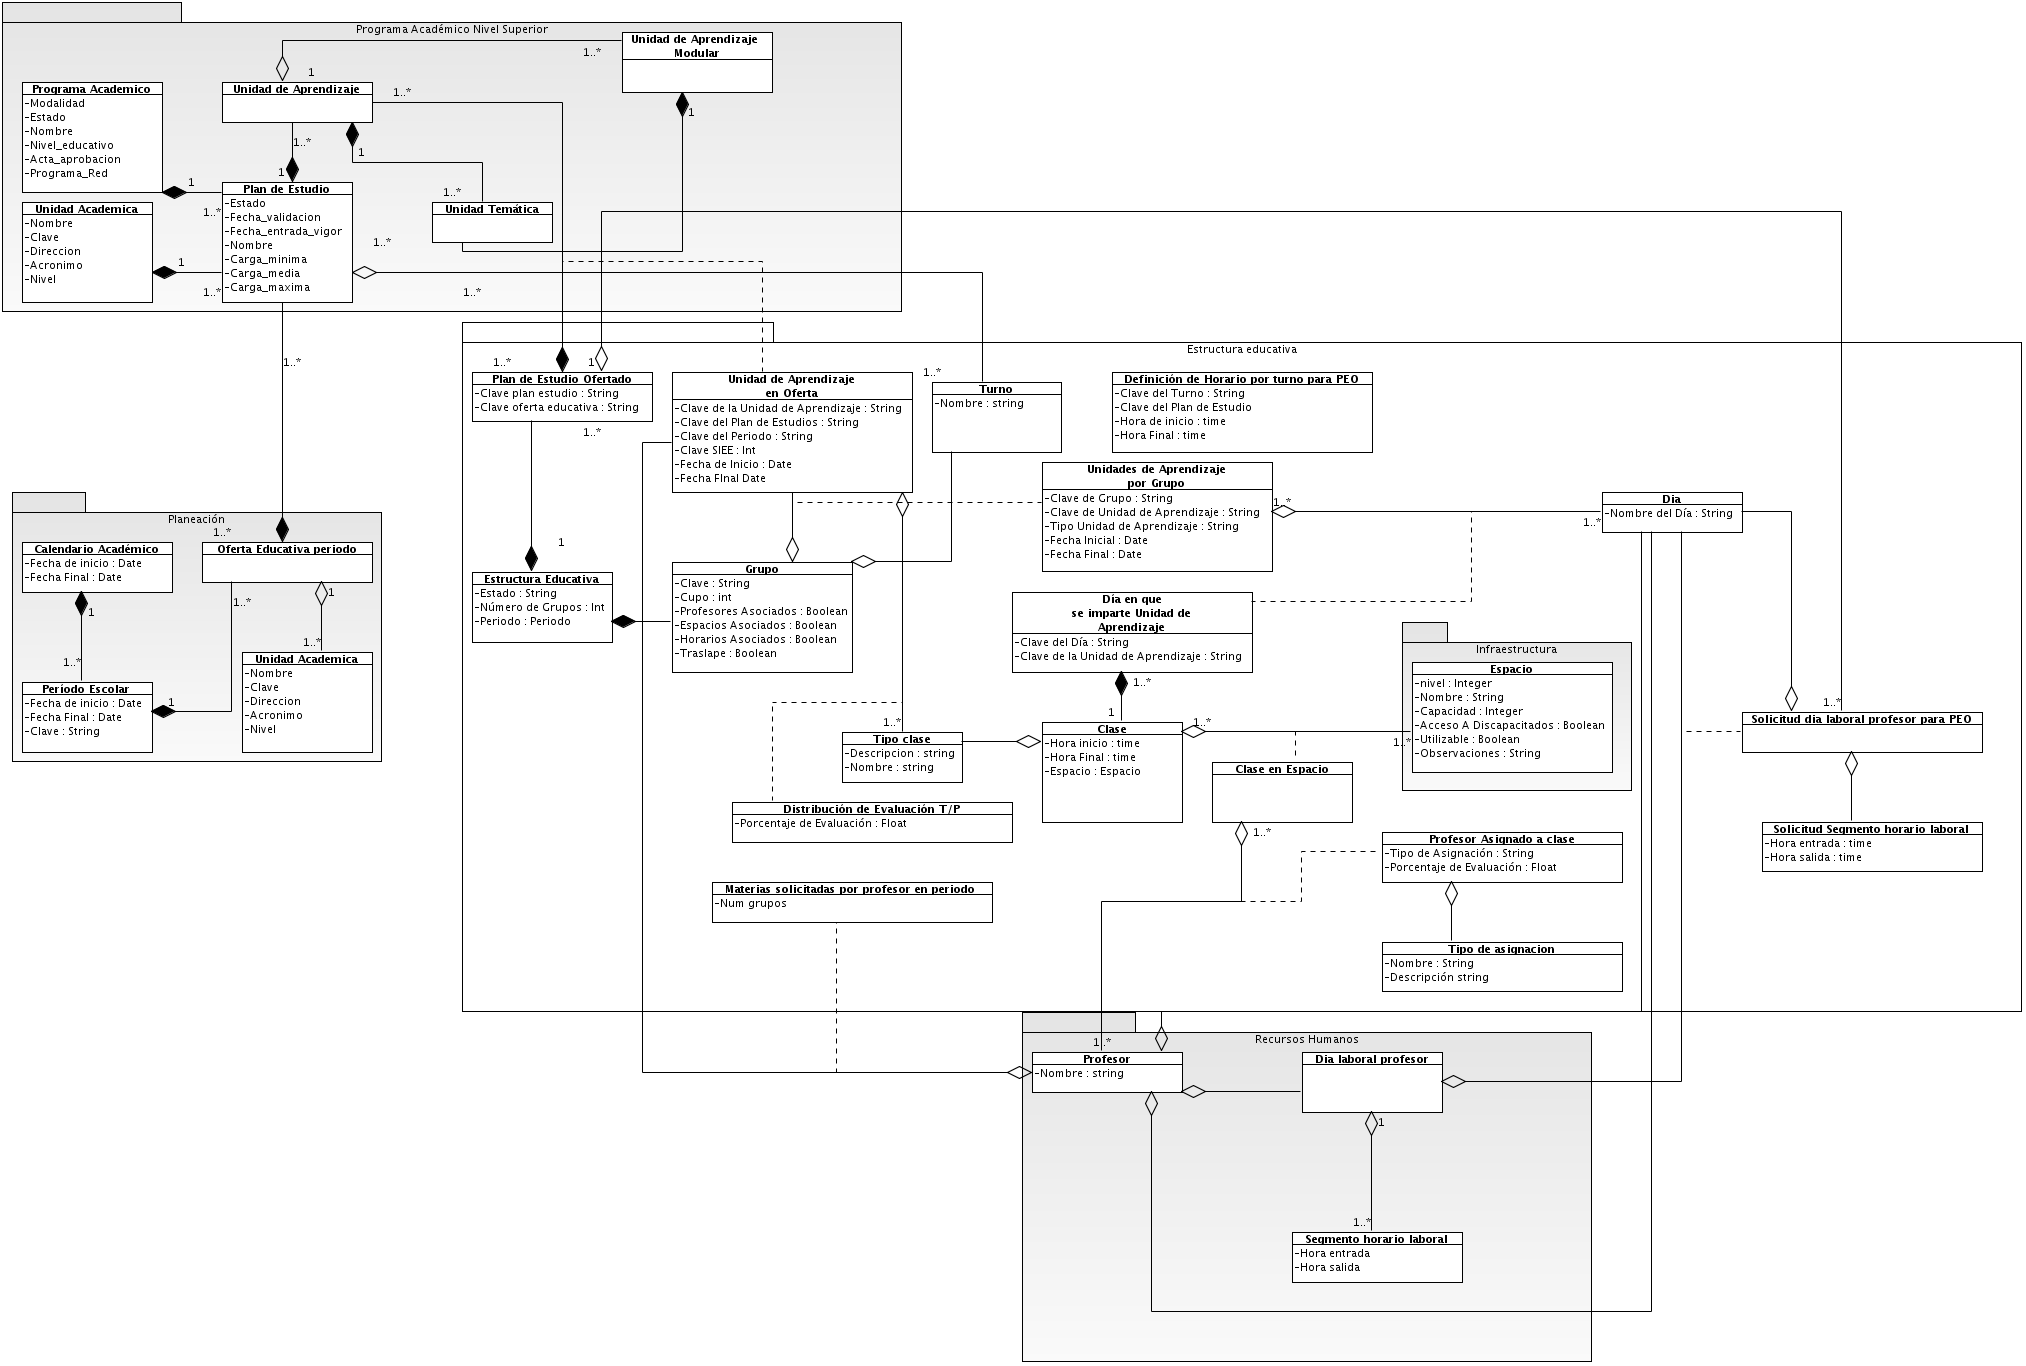
\includegraphics[width=\textwidth]{negocio/images/ModeloDeInformacion_EstructuraEducativa}}
		\label{fig:infoEstructuraEducativa}
		\caption{Modelo de Información de Estructura Educativa}
	\end{center}
\end{figure}

%---------------------------------------Entidad plan de estudio Ofertado
\begin{cdtEntidad}{PlanDeEstudioOfertado}{Plan de Estudio Ofertado}
	\brAttr{clavePlanOfertado}{Clave del plan de estudios}{Cadena}{Es la cadena que identifica al plan de estudios que será ofertado.}{\datRequerido}
	\brAttr{claveOfertaEducativa}{Clave de la oferta educativa}{Cadena}{Es la cadena que identifica a la oferta educativa del período en que se ha comenzado a trabajar.}{\datRequerido}
	\cdtEntityRelSection
	\brRel{\brRelComposition}{\refElem{UnidadDeAprendizaje}}{De un \refElem{PlanDeEstudioOfertado} se seleccionarán las Unidades de Aprendizaje que se ofrecerán en un periodo.}
	\brRel{\brRelAgregation}{\refElem{UnidadDeAprendizajeModular}}{Una \refElem{tUnidadDeAprendizajeModular} de un \refElem{PlanDeEstudioOfertado} es seleccionada para impartirse en un período.}
	\brRel{\brRelComposition}{\refElem{EstructuraEducativa}}{Una \refElem{EstructuraEducativa} se compondrá de un \refElem{PlanDeEstudioOfertado} o de varios para un período escolar.}
	
	\brRel{\brRelAgregation}{\refElem{Turno}}{Un \refElem{PlanDeEstudioOfertado} impartirá sus unidades de aprendizaje en oferta en diferentes turnos dentro de una unidad académica.}
\end{cdtEntidad}

%----------------------------------------Estructura Educativa
\begin{cdtEntidad}{EstructuraEducativa}{Estructura Educativa}
	\brAttr{estado}{Estado actual}{Estado}{Indica el estado actual de una \refElem{tEstructuraEducativa} con base en la máquina de estados \refIdElem{SM-EE}.}{\datRequerido}
	
	\brAttr{numeroDeGrupos}{Número de grupos}{Entero}{Indica el número de grupos son creados para una \refElem{EstructuraEducativa}}{\datOpcional}
	
	\brAttr{periodo}{Periodo}{Periodo}{Indica el período del Instituto para el cual es aplicable la \refElem{EstructuraEducativa}.}{\datRequerido}
	
	\cdtEntityRelSection
	
	\brRel{\brRelComposition}{\refElem{Grupo}}{Una \refElem{EstructuraEducativa} esta compuesta de varios grupos donde se imparten las unidades de aprendizaje por docentes interinos, de base, invitados o externos.}
	
	\brRel{\brRelComposition}{\refElem{PlanDeEstudioOfertado}}{Una \refElem{EstructuraEducativa} se compondrá de un \refElem{PlanDeEstudioOfertado} o de varios para un período escolar.}
	
	\brRel{\brRelAgregation}{\refElem{Estado}}{Una \refElem{EstructuraEducativa} cambiará su \refElem{estado} a lo largo de su planificación y aprobación esto es con base en la máquina \refIdElem{SM-EE}.}
	
\end{cdtEntidad}


%-----------------------------------------Estado
\begin{cdtEntidad}{Estado}{Estado}
	\brAttr{nombre}{Nombre}{Frase}{Indica el nombre del estado en que se encuentra una estructura educativa, un elemento de una estructura educativa o un profesor de una estructura educativa.}{\datRequerido}
	
	\brAttr{descripcion}{Descripción}{Frase}{Texto breve que tiene como propósito explicar que cosas suceden en un estado.}{\datRequerido}
	\cdtEntityRelSection
	
	\brRel{\brRelAgregation}{\refElem{EstructuraEducativa}}{Una \refElem{EstructuraEducativa} cambiará su \refElem{Estado} a lo largo de su planificación y aprobación esto es con base en la máquina \refIdElem{SM-EE}.}
\end{cdtEntidad}

%-----------------------------------------Unidad de Aprendizaje en Oferta

\begin{cdtEntidad}{UnidadDeAprendizajeEnOferta}{Unidad de Aprendizaje en Oferta}
	\brAttr{claveUnidadDeAprendizaje}{Clave de la unidad de aprendizaje}{Palabra}{Es la clave con la que se registró a la \refElem{tUnidadDeAprendizaje} de un \refElem{PlanDeEstudio}}{\datRequerido}
	
	\brAttr{clavePlanOfertado}{Clave del plan de estudios}{Palabra}{Es la clave que identifica al plan de estudios que será ofertado.}{\datRequerido}
	
	\brAttr{clavePeriodo}{Clave del periodo}{Palabra}{Es la clave con la que se identifica al período escolar en que se impartirá la unidad de aprendizaje en oferta.}{\datRequerido}
	
	\brAttr{claveSIEE}{Clave del SIEEE}{Entero}{Es la clave que se le asignó a la unidad de aprendizaje cuando fue registrada en el SIEE.}{\datRequerido}
	
	\cdtEntityRelSection
	
	\brRel{\brRelAgregation}{\refElem{Grupo}}{Una \refElem{UnidadDeAprendizajeEnOferta} se imparte en varios grupos.}
\end{cdtEntidad}

%--------------------------------------------Grupo

\begin{cdtEntidad}{Grupo}{Grupo}
	\brAttr{clave}{Clave}{Palabra}{Es la clave que el \refElem{UAResponsableEstructuraEducativa} detallará para determinar la etiqueta que le corresponda a un grupo o a varios para identificarlo de los demás de acuerdo a las necesidades y particularidades de cada unidad académica.}{\datRequerido}
	
	\brAttr{cupo}{Cupo}{Entero}{Es el número que indica la capacidad de alumnos y/o aspirantes que el espacio albergará para el grupo.}{\datRequerido}
	
	\brAttr{profesoresAsociados}{Profesores Asociados}{Booleano}{Indica si un grupo tiene todos los profesores necesarios para cubrir las unidades de aprendizaje.}{\datOpcional}
	
	\brAttr{espaciosAsociados}{Espacios Asociados}{Booleano}{Indica si un grupo tiene todos los espacios necesarios para cubrir las unidades de aprendizaje}{\datOpcional}
	
	\brAttr{horariosAssociado}{Horarios Asocidos}{Booleano}{Indica si en un grupo se encuentran asignados los días y el horario en que se impartiran las unidades de aprendizaje.}{\datOpcional}
	
	\brAttr{traslape}{Traslape}{Booleano}{Indica si en un grupo se permite el traslape entre horarios.}{\datOpcional} 
\end{cdtEntidad}


%----------------------------------------- Turno

\begin{cdtEntidad}{Turno}{Turno}
	\brAttr{nombre}{Nombre}{Palabra}{Indica el nombre asignado a un turno, pudiendo ser \begin{Citemize}
			\item Matutino
			\item Vespertino
			\item Mixto
	\end{Citemize}}{\datRequerido}
	\brAttr{horaDeInicio}{Hora de Inicio}{F}{}{}
\end{cdtEntidad}